\documentclass[12pt,a4paper]{article}
\usepackage[utf8]{inputenc}
\usepackage[T1]{fontenc}
\usepackage[brazil]{babel}
\usepackage{lmodern}
\usepackage{geometry}
\usepackage{graphicx}
\usepackage{booktabs}
\usepackage{longtable}
\usepackage{array}
\usepackage{amsmath}
\usepackage{xcolor}
\usepackage{listings}
\usepackage{hyperref}
\usepackage{fancyhdr}
\geometry{left=3cm,right=2cm,top=2.5cm,bottom=2.5cm}
\hypersetup{colorlinks=true,linkcolor=black,urlcolor=blue,pdftitle={Transmissão confiável de texto e imagem via RF 433 MHz}}
\setlength{\parindent}{1.2cm}
\setlength{\parskip}{0.25em}
\pagestyle{fancy}
\fancyhf{}
\fancyhead[L]{ESP32 e RF 433 MHz}
\fancyhead[R]{Transmissão e Comunicação de Dados}
\fancyfoot[C]{\thepage}
\lstset{basicstyle=\ttfamily\small,breaklines=true,frame=single,columns=fullflexible,showstringspaces=false}

\begin{document}
\begin{titlepage}
\begin{center}
{\large INSTITUTO FEDERAL DE EDUCAÇÃO, CIÊNCIA E TECNOLOGIA DE MATO GROSSO\par}
\vspace{0.3cm}
{\large Curso de Engenharia da Computação\par}
\vfill
{\LARGE\bfseries TRANSMISSÃO CONFIÁVEL DE TEXTO E IMAGEM ENTRE ESP32 VIA RF 433 MHz\par}
\vspace{0.5cm}
{\large CRC-8, Stop-and-Wait e Selective Repeat com reconstrução no computador receptor\par}
\vfill
\begin{flushleft}
\textbf{Integrantes:} Luanna Rabelo; Isis Tosti; Sophia Metello\\
\textbf{Disciplina:} Transmissão e Comunicação de Dados\\
\textbf{Professor:} Ruy de Oliveira
\end{flushleft}
\vfill
CUIABÁ\\2026
\end{center}
\end{titlepage}

\begin{abstract}
Este trabalho apresenta um enlace entre duas placas ESP32 e dois computadores, com quatro módulos de radiofrequência de 433 MHz: um transmissor e um receptor em cada placa. O computador A envia texto ou uma imagem escolhida por caminho de arquivo; o ESP32 A transmite quadros pelo rádio; o ESP32 B confirma o recebimento pelo caminho reverso; e o computador B salva o objeto reconstruído. O OLED da placa B exibe texto e sinaliza a chegada de imagem. O protocolo usa codificação Manchester, quadros de até 21 bytes, CRC-8 para detectar quadros alterados, CRC-32 para conferir o objeto completo e duas alternativas de retransmissão: Stop-and-Wait e Selective Repeat com janela de quatro quadros. Foram auditados 37 logs locais, que incluem entregas de texto e imagem, dois ensaios de corrupção proposital com detecção de FCS e recuperação, além de tentativas interrompidas, perda de ACK e falhas de acesso à porta serial. Uma fotografia documenta o arranjo usado à distância estimada pelo grupo em 0,8 a 1,0 m. O requisito estrito de distância superior a 1 m e a avaliação com interferência externa controlada ainda exigem ensaios específicos.

\noindent\textbf{Palavras-chave:} ESP32; RF 433 MHz; CRC; ARQ; Manchester; imagem.
\end{abstract}
\tableofcontents
\newpage

\section{Introdução}
O enunciado da disciplina solicita comunicação exclusivamente por módulos RF entre dois ESP32, transmissão confiável de texto e pequenas imagens, exibição do texto no display receptor, FCS, descarte de quadros corrompidos, retransmissão e demonstração presencial \cite{projeto}. A montagem do grupo usa OLED SSD1306 no lugar do LCD indicado no enunciado; a aceitação dessa substituição deve ser confirmada com o docente.

O programa em Python atua apenas como interface USB local de cada ESP32. Não existe comunicação direta entre os computadores. A imagem é reconstruída e salva no computador receptor, sem ocupar o OLED. O código atual oferece texto, fotografia colorida compactada e imagem monocromática rápida. A opção de enviar o arquivo original foi retirada da interface a pedido do grupo.

\section{Objetivos}
\subsection{Objetivo geral}
Implementar e demonstrar uma comunicação confiável de texto e imagem entre dois ESP32 usando somente rádio de 433 MHz entre as placas.

\subsection{Objetivos específicos}
\begin{itemize}
\item definir o quadro \texttt{FLAG|TYPE|SEQ|LEN|DATA|FCS}, com até 21 bytes;
\item detectar e descartar quadros alterados com CRC-8;
\item recuperar perdas com Stop-and-Wait ou Selective Repeat, escolhidos antes de cada envio;
\item confirmar o objeto completo com tamanho e CRC-32;
\item mostrar texto no OLED e salvar imagens no computador receptor;
\item registrar transmissões, confirmações, retransmissões e resultados nos dois computadores.
\end{itemize}

\section{Arquitetura e montagem}
Cada protoboard contém um ESP32, um módulo TX e um módulo RX de 433 MHz. O TX da placa A chega ao RX da B; o TX da B devolve ACK ao RX da A. Ambos os computadores usam USB somente para conversar com seu próprio ESP32. Assim, as mensagens de aplicação e os ACKs atravessam o rádio.

\begin{center}
\fbox{\parbox{0.9\linewidth}{\centering
PC A $\overset{\text{USB}}{\longleftrightarrow}$ ESP32 A $\xrightarrow{\text{RF DATA/END}}$ ESP32 B $\overset{\text{USB}}{\longleftrightarrow}$ PC B\\[0.5em]
ESP32 A $\xleftarrow{\text{RF ACK}}$ ESP32 B \qquad ESP32 B $\rightarrow$ OLED (texto)
}}
\end{center}

\begin{table}[h]
\centering
\caption{Conexões adotadas nas duas placas.}
\begin{tabular}{lll}
\toprule
Ligação & Placa A & Placa B \\
\midrule
DATA do transmissor RF & GPIO 26 & GPIO 26, para ACK \\
DATA do receptor RF & GPIO 27, para ACK & GPIO 27 \\
OLED I\textsuperscript{2}C & não instalado & SDA 21, SCL 22 \\
GND e alimentação & conforme os módulos & conforme os módulos \\
\bottomrule
\end{tabular}
\end{table}

Os GPIO 21 e 22 são uma configuração I\textsuperscript{2}C usual para ESP32 no ambiente Arduino \cite{arduinoi2c}. O programa tenta os endereços \texttt{0x3C} e \texttt{0x3D} do OLED. A tensão do sinal que entra em cada ESP32 deve ser compatível com 3,3 V. O modelo exato e a tensão nominal dos módulos RF utilizados precisam ser conferidos na peça antes de reproduzir a montagem. A fotografia da Figura~\ref{fig:oled} documenta o display da protoboard B; ela não permite verificar todas as ligações de rádio.

\begin{figure}[h]
\centering
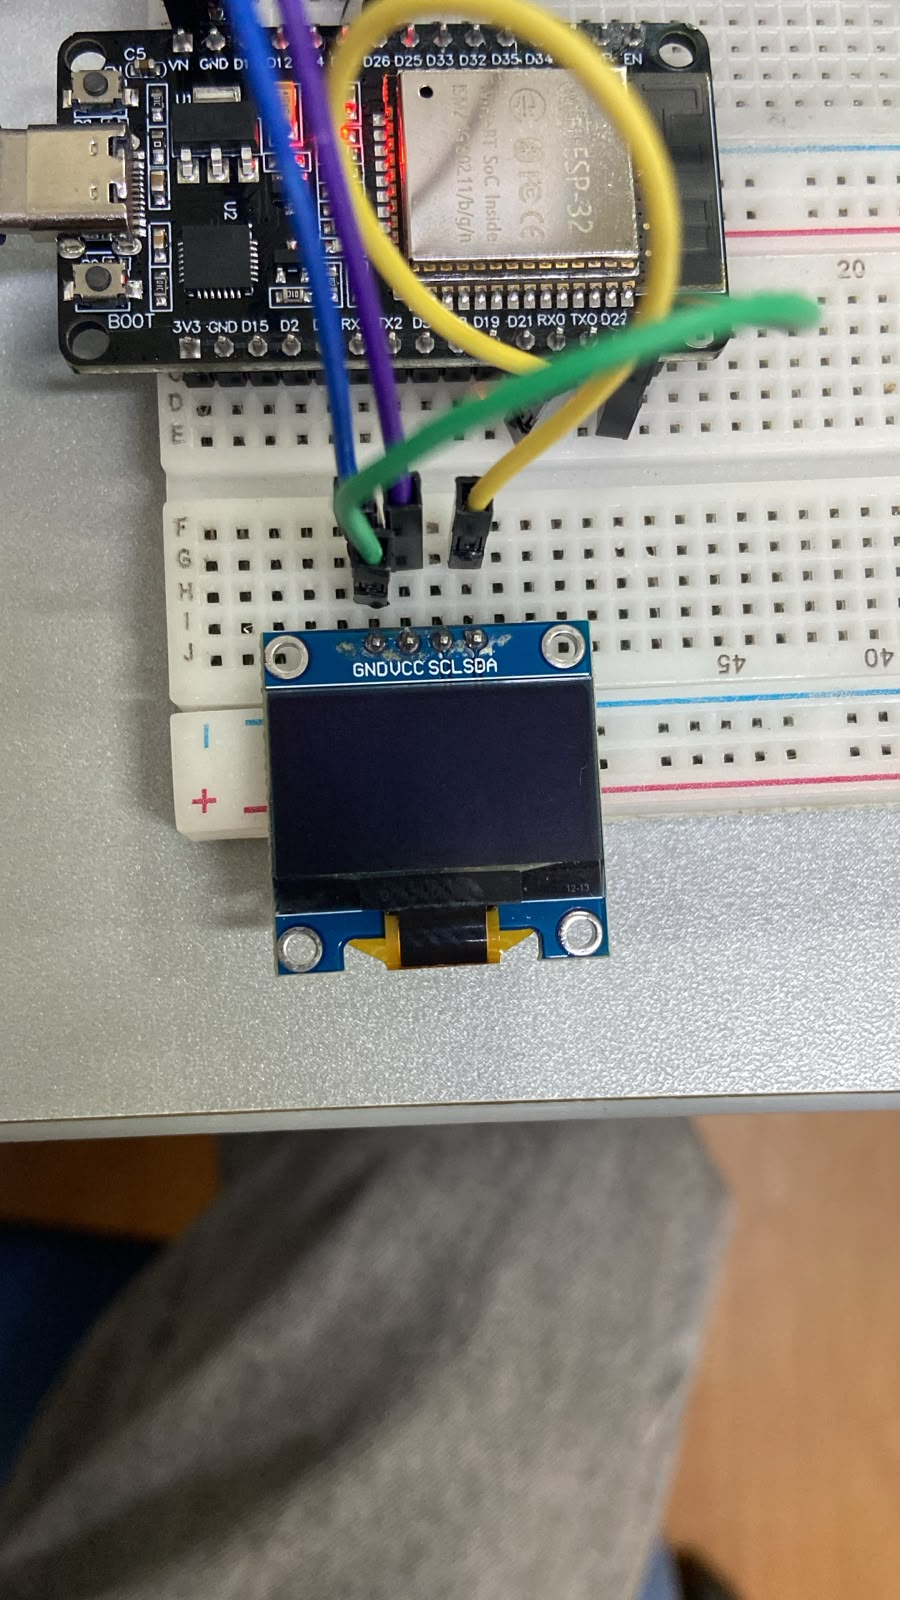
\includegraphics[height=6.0cm,keepaspectratio]{figuras/montagem_oled.png}
\caption{Detalhe da montagem do ESP32 e OLED fornecido pelo grupo.}
\label{fig:oled}
\end{figure}

\section{Formato do quadro e codificação física}
O enlace usa transmissão RF bruta, sem RadioHead. Cada bit é codificado em duas metades Manchester de 5 ms, resultando em 10 ms por bit. Antes do quadro, o firmware envia preâmbulo e sincronismo \texttt{0xD391}. Esses elementos pertencem à camada física e não entram nos 21 bytes máximos do quadro da Figura 2 do enunciado.

\begin{table}[h]
\centering
\caption{Quadro lógico transmitido pelo rádio.}
\begin{tabular}{llll}
\toprule
Campo & Bytes & Valor ou faixa & Função \\
\midrule
FLAG & 1 & \texttt{0x7E} & início \\
TYPE & 1 & 1, 2 ou 3 & DATA, ACK ou END \\
SEQ & 1 & 0 a 255 & sequência/base \\
LEN & 1 & 0 a 16 & comprimento de DATA \\
DATA & 0 a 16 & bytes & carga e controle \\
FCS & 1 & CRC-8 & verificação \\
\bottomrule
\end{tabular}
\end{table}

O maior quadro contém $1+1+1+1+16+1=21$ bytes. O CRC-8 cobre \texttt{TYPE}, \texttt{SEQ}, \texttt{LEN} e os \texttt{LEN} bytes de \texttt{DATA}; não cobre \texttt{FLAG} nem o próprio FCS. DATA transporta dez bytes do objeto e seis bytes de controle: identificador de sessão (4), informação da rodada (1) e base da rodada (1). O primeiro fragmento do objeto contém tipo (1), tamanho (2) e CRC-32 (4). Os tipos de uso atual são texto UTF-8, JPEG colorido compacto e pixels monocromáticos 32$\times$32. O preenchimento do último quadro não participa do CRC-32.

\section{Detecção e recuperação de erros}
\subsection{Cálculo do FCS}
Foi escolhido CRC-8 com polinômio $x^8+x^2+x+1$ (representação hexadecimal \texttt{0x07}), registrador inicial zero, sem reflexão e sem XOR final. Para cada byte protegido, o algoritmo faz XOR com o acumulador e repete oito vezes:
\begin{equation}
c_{j+1}=\begin{cases}
((c_j\ll 1)\oplus\texttt{0x07})\bmod 256,&\text{se o bit mais alto de }c_j\text{ era 1};\\
(c_j\ll 1)\bmod 256,&\text{caso contrário.}
\end{cases}
\end{equation}
Como verificação independente da rotina, a sequência ASCII \texttt{123456789} produz \texttt{0xF4}. O receptor recalcula o FCS sobre os bytes recebidos; se diferir do byte anexado, descarta o quadro e não confirma aqueles dados. O CRC-32 do objeto completo é uma segunda verificação antes de entregar texto ou imagem ao computador.

\subsection{Stop-and-Wait}
O transmissor envia um DATA, espera o ACK do mesmo número e repete o quadro após o tempo limite se a confirmação não chegar. O receptor reconhece uma duplicata e responde novamente, evitando duplicar bytes quando apenas o ACK se perde. Depois de todos os DATA, o transmissor envia END; o receptor verifica quantidade de quadros, comprimento e CRC-32, responde com ACK e entrega o objeto uma única vez.

\subsection{Selective Repeat}
O transmissor mantém janela de até quatro sequências. O receptor aceita quadros fora de ordem, armazena cada sequência uma única vez e devolve um mapa de bits no ACK: cada bit confirma independentemente uma posição relativa à base da rodada. O transmissor retransmite somente as posições ainda não confirmadas. Há 200 ms entre DATA de uma rodada, para dar tempo de recuperação aos módulos RF. A janela deslizante é definida pelo primeiro quadro pendente; não depende de o anterior ter chegado em ordem para armazenar os posteriores.

\subsection{Erro proposital}
A interface dispõe do comando \texttt{x}, que altera um byte de um DATA na primeira tentativa \emph{depois} de calcular o FCS. O receptor detecta a divergência, registra \texttt{FCS INVALIDO}, descarta o quadro e não confirma aquele fragmento. O transmissor esgota o tempo de espera e o reenvia. A Seção~\ref{sec:erro_observado} documenta dois ensaios efetivamente registrados, um em cada sentido durante o desenvolvimento. Trata-se de corrupção deliberada dos bytes transmitidos pelo firmware, não de uma medida de interferência eletromagnética externa.

\section{Software e reprodução}
O pacote contém \texttt{tx\_final.ino}, \texttt{rx\_final.ino}, biblioteca comum \texttt{RadioProjeto} e \texttt{projeto\_rf.py}. Os dois sketches são separados e definem se a placa usa OLED. O mesmo Python roda nos dois computadores, conectando-se a uma porta COM local a 115200 bit/s. O programa salva objetos e logs na pasta \texttt{recebidos}. O envio por caminho de arquivo ocorre no PC A; a recepção é reconstruída no PC B. O caminho digitado não é transmitido: o Python lê e prepara os bytes da imagem antes de enviá-los ao ESP32.

Para reproduzir, instalam-se as bibliotecas Adafruit GFX, Adafruit SSD1306 e RadioProjeto na Arduino IDE, grava-se o sketch TX na placa A e o RX na B, conecta-se cada computador ao seu ESP32 e inicia-se \texttt{projeto\_rf.py} em ambos. Com o monitor serial fechado, seleciona-se a COM local. Na interface, \texttt{s} escolhe Stop-and-Wait, \texttt{r} escolhe Selective Repeat, \texttt{t} envia texto e \texttt{i} solicita o caminho da imagem. No modo imagem, Enter cria JPEG colorido de até 32$\times$32; \texttt{m} cria 128 bytes de pixels em preto e branco. O Python do receptor precisa ficar aberto durante o envio para salvar o arquivo.

\section{Metodologia experimental}
Os registros usados foram produzidos em 24/11/2026 com dois ESP32 conectados ao mesmo computador por portas COM diferentes, mantendo o enlace entre placas por módulos RF. Foram escolhidos envios de texto e imagem e os modos Stop-and-Wait e Selective Repeat. O programa registra horário, tipo, tamanho, algoritmo, SHA-256 da carga, eventos de quadro/ACK e duração até \texttt{@FIM}. No receptor, registra \texttt{RX END | CRC-32 do objeto conferido}, caminho do arquivo salvo e SHA-256 recebido.

As portas COM não identificam permanentemente as placas; a confirmação de papel é a resposta \texttt{@PRONTO RF1 A} ou \texttt{B}. Alguns logs históricos mostram as duas placas como A após uma gravação equivocada. Foram escolhidos apenas pares de logs em que o conteúdo e o SHA-256 coincidem para sustentar as conclusões de entrega. Uma confirmação \texttt{@FIM} registra que o transmissor recebeu o ACK final do objeto, mas o arquivo no PC B depende de o Python receptor estar ativo.

\section{Resultados e evidências}
\begin{table}[h]
\centering
\caption{Exemplos verificados nos logs locais. Duração é a informada pelo transmissor.}
\begin{tabular}{p{3.4cm}p{1.7cm}p{1.2cm}p{1.7cm}p{4cm}}
\toprule
Objeto e horário & Modo & Bytes & Duração & Evidência de entrega \\
\midrule
Texto, 09:01--09:04 & S & 20 & 131,294 s & SHA-256 igual nos dois lados; arquivo TXT \\
JPEG compacto, 08:26--08:33 & S & 664 & 392,278 s & SHA-256 igual; arquivo JPG \\
Texto, 08:34--08:35 & R & 42 & 49,932 s & SHA-256 igual; arquivo TXT \\
Monocromática, 08:24--08:25 & S & 128 & 70,940 s & SHA-256 igual; arquivo PNG \\
\bottomrule
\end{tabular}
\end{table}

No exemplo de texto das 09:01, o SHA-256 em TX e RX foi \texttt{5775dfb21e9f90c20c2471d3ff23a9187719dd3aba51f86f8f5b2b8fff1b6720}. No JPEG de 664 bytes, foi \texttt{1b2042bdaa0b1f05cf1ec7b77ff2ad7165aec01666def3c5bf074fcd30565c85}. A coincidência comprova a igualdade dos bytes preparados pelo Python e salvos após a transmissão, além da checagem CRC-32 realizada pelo ESP32 B. A Figura~\ref{fig:recebida} mostra o JPEG reconstruído; sua resolução foi reduzida deliberadamente para diminuir o tempo de rádio.

\begin{figure}[h]
\centering
\fbox{
\includegraphics[width=4cm]{figuras/imagem_recebida.jpg}}
\caption{JPEG colorido recebido e salvo no computador receptor (arquivo de 664 bytes).}
\label{fig:recebida}
\end{figure}

Os logs contêm \texttt{Timeout | reenviando o que ficou sem ACK} e \texttt{RETX DATA}, demonstrando recuperação em tentativas com perda de confirmação. Em um teste anterior de texto com três quadros, o Stop-and-Wait concluiu em 56,684 s e o Selective Repeat concluiu em 124,827 s, mas eram mensagens diferentes e não constituem uma comparação controlada de desempenho. O Selective Repeat também entregou um texto de 42 bytes em 49,932 s. Portanto, ambos funcionaram; não se afirma superioridade de velocidade sem repetir a mesma carga nas mesmas condições.

A distância relatada pelo grupo foi de aproximadamente 80 cm a 1 m. O requisito do enunciado é \emph{superior} a 1 m, ainda não verificado. Há ensaio registrado com corrupção proposital e recuperação, porém não há medição documentada de ruído externo. A ocorrência de timeout e retransmissão demonstra recuperação de perdas em algumas sessões, mas não quantifica a tolerância a uma fonte externa de interferência controlada.

\section{Auditoria completa dos registros de execução}
\label{sec:auditoria}
Para distinguir os resultados demonstrados das impressões obtidas durante a montagem, foram examinados todos os 37 arquivos locais com nome \texttt{log\_COM*.txt} disponíveis até o encerramento da coleta. Esses arquivos são recortes sucessivos das portas seriais COM3 e COM5, e não 37 experimentos independentes: uma mesma bancada foi aberta e reiniciada várias vezes, alguns arquivos não têm par no outro computador e determinados envios começaram antes do fim da captura. As contagens da Tabela~\ref{tab:auditoria} são de \emph{eventos registrados}, sem normalização por tempo, carga, distância ou versão do firmware. Elas servem para tornar rastreável a revisão do conjunto, não para estimar uma taxa de erro do canal.

\begin{table}[h]
\centering
\caption{Inventário de eventos nos 37 logs locais (24/11/2026).}
\label{tab:auditoria}
\begin{tabular}{p{8cm}r}
\toprule
Indicador extraído literalmente dos arquivos & Ocorrências \\
\midrule
Logs iniciados com placa identificada como A / B & 29 / 8 \\
Comandos \texttt{ENVIO} registrados (S / R) & 60 (38 / 22) \\
\texttt{@FIM} / \texttt{@CANCELADO} / tentativa sem desfecho no mesmo arquivo & 29 / 18 / 13 \\
Objetos efetivamente salvos com registro \texttt{RECEBIDO:} & 16 \\
Linhas de timeout / \texttt{RETX DATA} & 1160 / 1672 \\
Linhas \texttt{ERRO INJETADO} / \texttt{FCS INVALIDO} & 2 / 2 \\
Avisos de desconexão da porta serial & 12 \\
\bottomrule
\end{tabular}
\end{table}

Os 13 envios sem desfecho no mesmo arquivo não devem ser automaticamente chamados de falhas definitivas: houve encerramento ou troca do terminal e falta o par remoto em parte do histórico. Do mesmo modo, os 29 \texttt{@FIM} não equivalem a 29 arquivos comprovadamente salvos neste acervo. O contador de retransmissões soma tentativas de DATA de tamanhos diferentes; uma imagem de 68 quadros naturalmente produz mais eventos que um texto de um quadro. A coexistência de confirmações e longas séries de timeout mostra um enlace \emph{intermitente} na bancada observada, mas a tabela não separa perda de DATA, perda do ACK, conflito de transmissão, alimentação ou problema da interface USB.

\subsection{Leitura cronológica dos ensaios}
No início da manhã, \texttt{log\_COM3\_20261124\_070220.txt} registrou texto de 23 bytes em Stop-and-Wait concluído em 56,684 s, com sete retransmissões de DATA. Um texto de 14 bytes em Selective Repeat terminou em 124,827 s após 33 retransmissões; outro envio R foi cancelado. A imagem monocromática de 128 bytes em S terminou em 65,196 s sem retransmissão de DATA nessa sessão. Houve ainda uma tentativa histórica de 1999 bytes no formato de arquivo original, que avançou por muitos quadros, mas foi cancelada; a opção de transmitir o original foi posteriormente removida da interface, conforme o escopo definido pelo grupo. A passagem pelo número de sequência 100 nessa tentativa não caracteriza um limite de 100 quadros do protocolo.

Entre 07:48 e 08:35 apareceram evidências dos dois lados: a placa B recebeu texto e confirmou duplicatas em \texttt{log\_COM5\_20261124\_074852.txt}; depois, o conjunto \texttt{log\_COM3\_20261124\_082016.txt} e \texttt{log\_COM5\_20261124\_082007.txt} registrou JPEG de 664 bytes, texto em R e imagem monocromática. Os hashes coincidentes e os arquivos salvos sustentam a integridade desses objetos. Porém, nesse segundo par ambos os terminais se identificaram como A, situação de desenvolvimento causada por gravação de papel incorreto. O enlace RF e a reconstrução foram exercitados, mas esse par não serve como demonstração do OLED da placa B.

Nos registros das 08:48, os dois lados ainda apareciam como A; a identificação B voltou a constar no log COM5 iniciado às 08:57. A distinção é relevante porque uma placa gravada como A não inicializa o OLED pelo caminho reservado a B. Mesmo após corrigir o papel, algumas tentativas entre 08:58 e 09:00 foram canceladas sem ACK. Portanto, a correção de sketch era necessária para o display, mas não explica sozinha toda a instabilidade de rádio.

Às 09:01, um texto de 20 bytes no modo S terminou em 131,294 s e foi salvo na placa B com o mesmo SHA-256 do emissor. Mais tarde, às 09:23 e 09:25, ocorreram os dois ensaios com erro deliberado descritos adiante. A partir das 10:38, os logs voltam a mostrar períodos sem ACK, alguns envios concluídos e desconexões seriais. Na série vespertina entre 17:20 e 19:01 há várias sessões de textos curtos com dezenas ou centenas de retransmissões sem conclusão registrada; outras foram canceladas. Exemplos incluem 83 \texttt{RETX DATA} sem ACK em uma tentativa iniciada às 17:49 e 124 retransmissões de um texto de 12 bytes iniciado às 18:05, antes do cancelamento às 18:17. Em contrapartida, textos R iniciados às 18:17 e 18:21 concluíram, respectivamente, em 96,730 e 100,070 s. O comportamento variável em uma mesma tarde impede interpretar o sistema como permanentemente funcional ou permanentemente inoperante.

No log iniciado às 19:22, já após a restrição de novos envios à placa A, foram registrados oito \texttt{@FIM} sucessivos: textos em S e R, uma imagem monocromática de 128 bytes em R e um JPEG de 664 bytes em S. O JPEG concluiu em 459,258 s com 27 retransmissões de DATA; o texto R de 9 bytes terminou em 10,088 s sem retransmissão. Uma tentativa posterior de JPEG em R foi cancelada e outra estava em andamento quando o arquivo terminou. Como o log da placa B nessa sessão não foi fornecido, os \texttt{@FIM} demonstram ACK final recebido por A, mas não documentam o caminho de arquivo efetivamente salvo no outro computador. Essa distinção é importante para uma apresentação em dois PCs.

\subsection{Detecção e recuperação do erro injetado}
\label{sec:erro_observado}
O par \texttt{log\_COM5\_20261124\_090135.txt} / \texttt{log\_COM3\_20261124\_090130.txt} fornece a sequência completa de dois testes históricos. No primeiro, B iniciou o envio de 23 bytes às 09:23:26. Na tentativa inicial de \texttt{SEQ=1}, às 09:23:42, o emissor anotou \texttt{ERRO INJETADO}; A marcou \texttt{FCS INVALIDO} às 09:23:44. Sem ACK desse fragmento, B registrou timeout e \texttt{RETX DATA} às 09:23:48. A aceitou o novo \texttt{SEQ=1}, verificou o CRC-32 do objeto às 09:23:58, e B recebeu \texttt{@FIM 33724} às 09:24:00. O SHA-256 do texto recebido foi \texttt{5a3236c3f442e1ca0ef706d73e7b320bb22cdc045eba9f1dda028e8dfc7bb125}, igual ao do envio.

No segundo teste, A iniciou 23 bytes em S às 09:25:12. O \texttt{SEQ=1} saiu com \texttt{ERRO INJETADO} às 09:25:17, B anotou \texttt{FCS INVALIDO} às 09:25:19, A reenviou às 09:25:23 e recebeu ACK às 09:25:27. B verificou o CRC-32 e salvou o texto às 09:25:35; A registrou \texttt{@FIM 22244}. O SHA-256 coincidente foi \texttt{da24097e87a40e10d41b66567c45fd2649f508e4b68608c221992a024fd59c92}. A injeção foi feita uma só vez, de modo que a retransmissão portou o byte correto. Esses dois episódios demonstram detecção, descarte, recuperação e entrega para a falha artificial especificada. O primeiro, com B transmitindo dados, pertence a uma versão anterior à regra atual de papéis; o segundo segue o sentido A--B.

\subsection{Distância fotografada e alcance demonstrado}
A Figura~\ref{fig:distancia} registra as duas montagens nas extremidades da bancada usada no ensaio. O grupo informou separação de aproximadamente 80 cm a 1 m. A imagem não contém trena, régua nem referência métrica confiável; assim, ela comprova o arranjo físico e a separação visual, mas não permite medir o vão com precisão. O enunciado solicita distância \emph{maior que 1 m}; uma estimativa que alcança no máximo 1 m não satisfaz essa desigualdade estrita. Portanto, o resultado positivo nesta bancada é reportado como funcionamento a 0,8--1,0 m, sem extrapolação para alcance maior.

\begin{figure}[h]
\centering
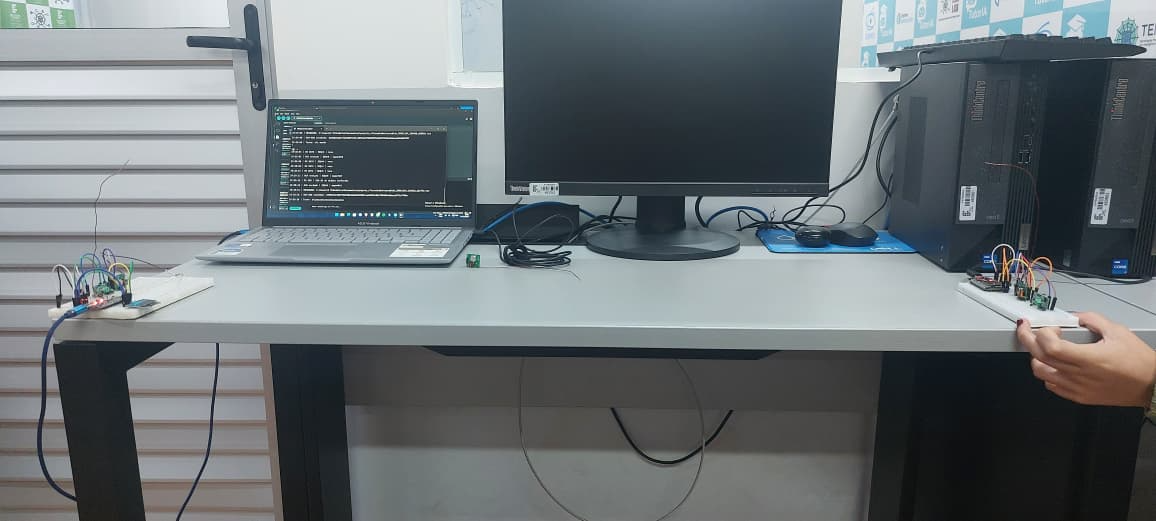
\includegraphics[width=0.95\linewidth,keepaspectratio]{figuras/distancia_bancada.png}
\caption{Montagens nas extremidades da mesa durante o ensaio. Distância aproximada de 0,8 a 1,0 m informada pelo grupo; a foto não contém escala para medição independente.}
\label{fig:distancia}
\end{figure}

\section{Falhas observadas, hipóteses e correções}
\label{sec:falhas}
\subsection{Longas esperas sem ACK}
O sintoma mais frequente de insucesso nos logs é a repetição de \texttt{Timeout | reenviando o que ficou sem ACK} seguida de \texttt{RETX DATA} do mesmo número de sequência. Em Stop-and-Wait, um único quadro sem confirmação impede o avanço; em Selective Repeat, o emissor pode continuar a confirmar outros elementos da janela, mas a base pendente bloqueia o progresso posterior. No exemplo de texto de 16 bytes iniciado às 18:33, o primeiro quadro acumulou 53 retransmissões sem ACK até o fim da captura. Esse padrão permite afirmar que A \emph{não observou uma confirmação válida}; ele não permite decidir, apenas pelo log de A, se B deixou de receber o DATA, se o ACK se perdeu no retorno, se a outra placa estava transmitindo em vez de escutar, ou se houve falha elétrica. Uma linha de timeout isolada também não é sinônimo de FCS inválido: muitos quadros degradados podem falhar antes de formar um quadro completo reconhecível.

\subsection{Disputa entre iniciações de envio}
Durante o desenvolvimento, ambos os programas permitiam iniciar objetos. O firmware, ao entrar no estado \texttt{enviando}, processava ACKs da própria sessão e ignorava DATA ou END recebidos. Se A e B começassem objetos ao mesmo tempo, cada placa poderia permanecer ocupada esperando resposta enquanto descartava o objeto da outra. Esse é um mecanismo de impasse identificado na revisão do código, coerente com algumas tentativas sem progresso, mas os logs incompletos não comprovam que ele foi a única causa de cada falha. A revisão adotada fixou o papel de aplicação: A inicia DATA/END e B recebe e devolve ACK; o Python impede a operação \texttt{t}/\texttt{i} na placa identificada como B. O rádio continua bidirecional para controle. A série posterior das 19:22 contém oito conclusões, um indício de melhora prática após a mudança. Como montagem, posição, alimentação e condições de RF não foram controladas entre as séries, não se atribui causalidade exclusiva à alteração do software.

\subsection{Temporização e custo da confiabilidade}
Na revisão do Selective Repeat, a pausa entre DATA sucessivos de uma rodada passou de 12 ms para 200 ms. O intervalo maior procura dar ao receptor mais tempo para terminar o processamento e a escuta antes da próxima emissão; o código atual também reserva 400 ms antes de responder com ACK, 250 ms depois de ACK e 3500 ms como limite de espera. O tempo de ocupação de rádio é elevado: cada bit Manchester contém duas metades de 5 ms, portanto um quadro lógico máximo de 21 bytes exige pelo menos $21\cdot 8\cdot 10\,\mathrm{ms}=1{,}68\,\mathrm{s}$ só para seus bits, além de preâmbulo, sincronismo, cauda e períodos de guarda. O acréscimo de pausa reduz a taxa bruta em troca de uma margem operacional maior. Há percepção do grupo de melhora após o ajuste, mas não foi realizado ensaio comparativo que isolasse somente o valor 12/200 ms, com mesma carga, posição e versão restante do código. Por isso, o relatório registra a decisão e seu motivo, não um ganho percentual demonstrado.

\subsection{Falhas de USB, gravação e observabilidade}
Os 12 avisos de desconexão serial incluem erros de acesso à porta, como \texttt{ClearCommError failed} no log COM3 das 18:05. Isso aponta uma falha na comunicação entre PC e ESP32 ou na disponibilidade da COM naquele instante; não é evidência direta de perda no ar. Nesses casos, reiniciar o terminal, verificar o cabo e fechar outro programa que ocupe a porta são verificações necessárias antes de atribuir o problema ao módulo RF. Outra fonte de confusão ocorreu quando ambas as placas responderam \texttt{@PRONTO RF1 A}: os dados podiam circular, mas o firmware sem OLED não apresentaria texto na tela. A identificação do papel na abertura do terminal passou a ser uma verificação operacional obrigatória.

Há ainda uma limitação de observação: o ESP32 B pode enviar o ACK final e deixar a mensagem serial para o PC B, mas se o Python do receptor estiver fechado, o arquivo não aparecerá na pasta \texttt{recebidos}. O ACK final, portanto, comprova o término visto pelo transmissor e a verificação no firmware receptor; o arquivo salvo e o SHA-256 no segundo computador requerem o log da aplicação B. Na apresentação, manter ambos os terminais abertos e conferir tanto \texttt{@FIM} quanto \texttt{RECEBIDO:} evita declarar entrega ao PC com base em apenas um lado.

\begin{table}[h]
\centering
\caption{Relação entre sintoma, evidência disponível e alcance da conclusão.}
\begin{tabular}{p{3cm}p{4.2cm}p{5.2cm}}
\toprule
Sintoma & O que foi observado & Conclusão sustentada \\
\midrule
FCS inválido após \texttt{x} & Dois pares de logs, retransmissão e hash igual & Quadro corrompido foi descartado e o objeto acabou recuperado \\
Muitos timeouts & Repetição de DATA sem ACK observado & Houve falta de confirmação; causa específica do caminho RF não isolada \\
Ambas as placas como A & \texttt{@PRONTO RF1 A} em COM3 e COM5 & Papel incorreto para demonstrar OLED B nessa sessão \\
Erro \texttt{ClearCommError} & Desconexão registrada no terminal & Falha local da interface serial; não mede qualidade do RF \\
\texttt{@FIM} sem log B & Confirmação final no log A & Fim do protocolo observado por A; salvamento no PC B não documentado \\
\bottomrule
\end{tabular}
\end{table}

\section{Critérios do projeto e estado das evidências}
\begin{longtable}{p{5cm}p{3cm}p{5cm}}
\caption{Situação dos itens relevantes para a demonstração.}\label{tab:criterios}\\
\toprule
Item & Estado & Base da avaliação \\
\midrule
\endfirsthead
\toprule Item & Estado & Base da avaliação \\ \midrule
\endhead
Dois ESP32 e rádio entre placas & Demonstrado em bancada & Pares COM3/COM5 com recebimento e ACK; foto do arranjo \\
Texto e imagem no computador receptor & Demonstrado & Arquivos salvos, CRC-32 e SHA-256 correspondente em pares de logs \\
Stop-and-Wait e Selective Repeat & Demonstrado funcionalmente & Envios S e R concluídos; sem comparação controlada de desempenho \\
Erro intencional, FCS e recuperação & Demonstrado & Dois ensaios das 09:23 e 09:25 com \texttt{FCS INVALIDO}, retransmissão e entrega \\
Distância superior a 1 m & Pendente & Estimativa informada 0,8--1,0 m; foto sem escala \\
Ruído externo controlado & Pendente & Injeção de byte não equivale a interferência física controlada \\
Texto visível no OLED & Funcional segundo o grupo; registro visual pendente & Montagem OLED fotografada; não há foto final da frase exibida \\
Uso de OLED no lugar do LCD pedido & Confirmação docente pendente & Divergência de tipo de display em relação ao enunciado \\
Mesma carga S/R sob condições iguais & Pendente como comparação quantitativa & Amostras têm tamanhos, horários e condições diferentes \\
\bottomrule
\end{longtable}

\section{Limitações e próximos ensaios}
Cada DATA de 21 bytes, a 10 ms por bit Manchester, ocupa cerca de 1,68 s de transmissão lógica, além do preâmbulo, sincronismo, cauda, pausas e ACK. Por isso, imagens coloridas compactas de algumas centenas de bytes podem levar minutos. O modo monocromático é mais rápido, mas perde cor e detalhes. A foto JPEG recebida corresponde à versão compactada preparada no computador A, não ao arquivo de origem em resolução plena.

Para completar os critérios presenciais: medir e registrar distância \emph{maior} que 1 m com instrumento visível; repetir a mesma carga com S e R sob condições semelhantes e anotar tempo e retransmissões; registrar um ensaio de interferência física controlada, quando seguro e permitido no laboratório; fotografar o texto no OLED durante a entrega; e confirmar com o docente o uso do OLED em lugar do LCD. O teste \texttt{x}, antes pendente, já está documentado na Seção~\ref{sec:erro_observado}.

\section{Conclusão}
Foi implementado um enlace RF bidirecional de controle entre dois ESP32, com transmissão de texto e imagens do computador A ao B, CRC-8 por quadro, CRC-32 por objeto e dois métodos de ARQ. Os logs confirmam entregas de texto, PNG monocromático e JPEG compacto com SHA-256 correspondente nos dois computadores, inclusive após retransmissões. Dois ensaios históricos mostram corrupção proposital, descarte por FCS e posterior entrega. A mesma auditoria evidencia que a comunicação pode se tornar intermitente, com muitas retransmissões e sessões sem conclusão; o protocolo recupera certas perdas, mas não garante êxito quando o enlace ou a porta serial permanecem indisponíveis. A demonstração do texto no OLED foi informada pelo grupo como funcional, mas não há fotografia final do texto no display anexada. Distância superior a 1 m e ruído externo controlado permanecem pendentes de evidência.

\section{Disponibilidade dos arquivos}
O pacote de entrega contém código-fonte, instruções de montagem, este relatório em LaTeX e exemplos de logs e arquivos recebidos. O repositório deste projeto é \url{https://github.com/luannarabeloo/esp32-rf-433mhz-texto-imagem}. O repositório citado em conversas anteriores foi apenas referência e não faz parte desta entrega.

\begin{thebibliography}{9}
\bibitem{projeto} INSTITUTO FEDERAL DE MATO GROSSO. \emph{Projeto Final da Disciplina Transmissão e Comunicação de Dados: transmissão confiável via rádio}. Material da disciplina, 2026.
\bibitem{arduinoi2c} ESPRESSIF SYSTEMS. \emph{GPIO Matrix and Pin Mux -- Arduino ESP32 Documentation}. Disponível em: \url{https://docs.espressif.com/projects/arduino-esp32/en/latest/tutorials/io_mux.html}. Acesso em: 24 nov. 2026.
\bibitem{datasheet} ESPRESSIF SYSTEMS. \emph{ESP32-WROOM-32 Datasheet}. Disponível em: \url{https://documentation.espressif.com/esp32-wroom-32_datasheet_en.html}. Acesso em: 24 nov. 2026.
\end{thebibliography}
\end{document}
